\documentclass[12pt]{article}

\usepackage[margin=0.8in]{geometry}
\usepackage[utf8]{inputenc}
\usepackage{hyperref}
\usepackage{graphicx}
\usepackage{amsmath}
\usepackage{pgfplots}
\usepackage{xcolor}
\usepackage{listings}
\usepackage{amssymb} 

\lstset{language=[90]Fortran,
  basicstyle=\ttfamily,
  keywordstyle=\color[HTML]{B22222},
  commentstyle=\color[HTML]{555555},
  morecomment=[l]{!\ }% Comment only with space after !
}

\pgfplotsset{width=10cm,compat=1.9}
\graphicspath{{./img}}
\usepgfplotslibrary{external}

\title{Perceptron}
\author{Erick Alejandro Carrillo López}
\date{2023/04/03}

\begin{document}
\maketitle
\tableofcontents
\newpage

\section{How works?:}
\subsection{A real neuron:}
A real neuron, also known as a nerve cell, is a specialized cell that transmits
electrical and chemical signals in the nervous system.\\
At the most basic level, a neuron consists of a cell body, dendrites, and an axon.
The cell body contains the nucleus and other organelles, and serves as the metabolic center
of the neuron. Dendrites are thin, branching extensions that receive signals from other
neurons or sensory cells. The axon is a long, thin projection that carries signals away
from the cell body to other neurons or target cells.
\begin{figure}[h]
  \centering
  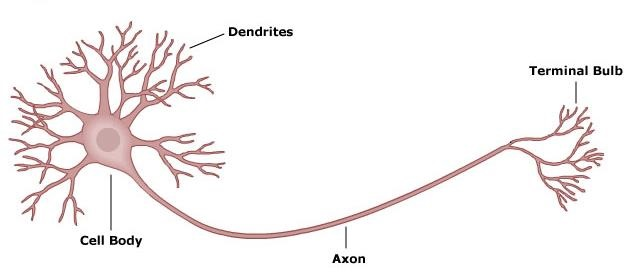
\includegraphics[scale = 0.5]{cell-body.jpg}
  \caption{Cell Body with its axon}
\end{figure}
Neurons communicate with each other through synapses, which are specialized
junctions between neurons. When an electrical signal, known as an action potential,
reaches the end of an axon, it triggers the release of neurotransmitter molecules, which diffuse
across the synapse and bind to receptors on the dendrites or cell body of the target neuron. This
binding can cause the target neuron to generate its own action potential, which propagates down its
axon to signal other neurons or target cells.
\begin{figure}[h]
  \centering
  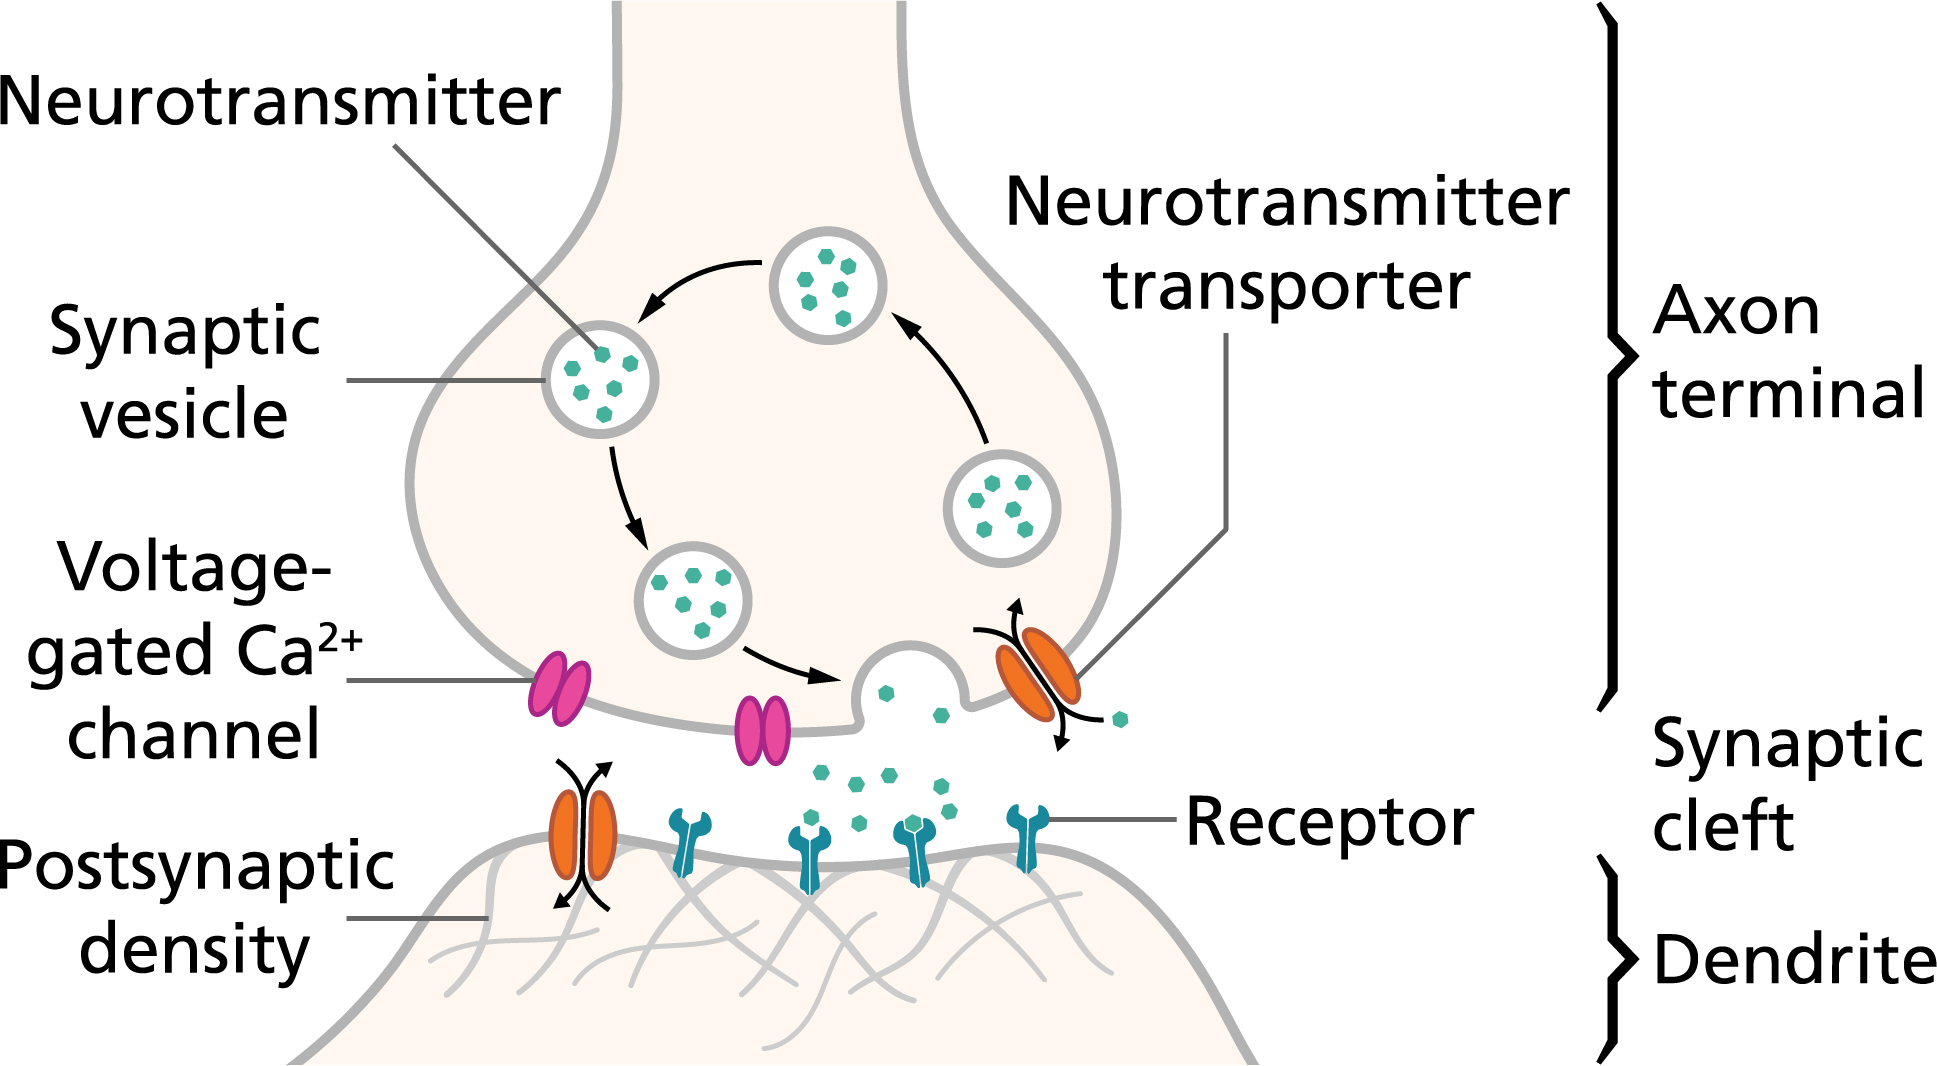
\includegraphics[scale = 0.19]{Synapse.jpg}
  \caption{Synapse}
\end{figure}

Neurons talk to each other across synapses. When an action potential reaches the
presynaptic terminal, it causes neurotransmitter to be released from the neuron into the synaptic
cleft, a 20–40nm gap between the presynaptic axon terminal and the postsynaptic dendrite
(often a spine).\\
After travelling across the synaptic cleft, the transmitter will attach to neurotransmitter
receptors on the postsynaptic side, and depending on the neurotransmitter released
(which is dependent on the type of neuron releasing it), particular positive (e.g. Na+, K+, Ca+)
or negative ions (e.g. Cl-) will travel through channels that span the membrane.
\subsection{The perceptron:}
The perceptron is a type of artificial neural network that is loosely modeled after the structure
and function of real neurons in the brain. The basic idea behind the perceptron is to use a
mathematical algorithm to simulate the behavior of a simplified neuron, which can then be used to
perform simple classification tasks.\\
The perceptron consists of an input layer, a set of weights, a summing or activation function,
and an output.
The input layer consists of one or more nodes, each of which represents a feature of the input data.
The weights are values that are assigned to each input node, which control the strength of the
connection between that node and the output.
\begin{figure}[h]
  \centering
  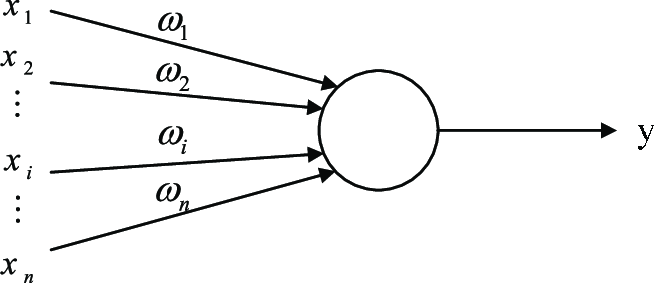
\includegraphics[scale = 0.5]{perceptron.png}
  \caption{Perceptron}
\end{figure}

The summing or activation function takes the weighted inputs and adds them together to produce a
single output
value. This output value is then compared to a threshold value, which determines whether the
perceptron will output a positive or negative value. If the output is positive, the perceptron
classifies the input as belonging to one class; if it is negative, the input is classified as
belonging to the other class.
\subsection{Perceptron parts:}
\begin{itemize}
\item \textbf{Input Nodes or Input Layer:} \\
  This is the primary component of Perceptron which accepts the initial data into the system for
  further processing. Each input node contains a real numerical value.
\item \textbf{Wight and Bias:} \\
  Weight parameter represents the strength of the connection between units. This is another most
  important parameter of Perceptron components. Weight is directly proportional to the strength of the
  associated input neuron in deciding the output. Further, Bias can be considered as the line of
  intercept in a linear equation.
\item \textbf{Activation Function:} \\
  These are the final and important components that help to determine whether the neuron will
  fire or not. Activation Function can be considered primarily as a step function.\\
  \textbf{Types of Activation functions:}
  \begin{itemize}
  \item Sign function.
  \item Step function.
  \item Sigmoid function.
  \end{itemize}
  \begin{figure}[h]
    \centering
    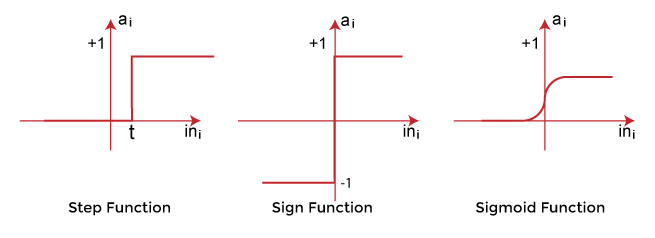
\includegraphics[scale = 0.5]{funcs.png}
    \caption{Types of activation functions}
  \end{figure}
\end{itemize}
\section{Códing the perceptron:}
\subsection{The Perceptron Algorithm:}
Perceptron model works in two important steps as follows.
\begin{enumerate}
\item In the first step first, multiply all input values with corresponding weight values and then add
  them to determine the weighted sum. Mathematically, we can calculate the weighted sum as follows.\\
  \[
    \sum_{i = 0}^{n}(weight_i \cdot input_i) = \sum_{i = 0}^{n}(w_i \cdot x_i) = w_0 \cdot x_0 + w_1 \cdot x_1
    + \cdots + w_n \cdot x_n
  \]\\
  Add a special term called bias 'b' to this weighted sum to improve the model's performance.\\
  \[
    \sum_{i = 0}^{n}(w_i \cdot x_i) + b
  \]
\item In the second step, an activation function is applied with the above-mentioned weighted sum,
  which gives us output either in binary form or a continuous value as follows.\\
  \[
    y = activation(\sum_{i = 0}^{n}(w_i \cdot x_i) + b) = activation(\vec{w} \cdot \vec{x} + b)
  \]
\end{enumerate}
At the end what we are doing here is a simple dot product of two vectors.
\[
  \sum_{i = 0}^{n}(w_i \cdot x_i) + b = \vec{w} \cdot \vec{x}
\]
Where.
\[
  \vec{w} = (b, w_1, \cdots, w_n)
\]
\[
  w_0 = b
\]
\[
  \vec{x} = (1, x_1, \cdots, x_n)
\]
\[
  x_0 = 1
\]
At the end we can think that this is hiperplane.

\begin{figure}[!hb]
  \centering
  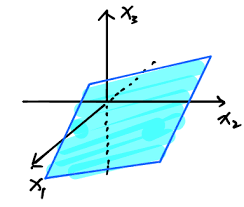
\includegraphics[scale = 1]{plane.png}
  \caption{A hyperplane}
\end{figure}

\subsection{From the perceptron algorithm to code:}
Firstly declare the threshold variable or bias variable,
this variable will be used as a threshold or bias for the activation function.
\begin{verbatim}
const threshold = 1.5
\end{verbatim}
After that declare two arrays the weights and inputs, the weights array is always initialized with random
values.
\begin{verbatim}
inputs = [1, 0, 1, 0, 1]
weights = [0.7, 0.6, 0.5, 0.3, 0.4]
\end{verbatim}
The weighted sum of the input values and weights by initializing a variable called sum to zero,
and then iterating over the input values and weights and adding the product of each input value
and weight to sum.
\begin{verbatim}
sum = 0.0
for (i = 0, i < inputs.length, i++)
    sum += inputs[i] * weights[i]
\end{verbatim}
And at the end just apply an activation function, a sign function to the weighted sum by checking
if sum is greater
than the threshold value of 1.5. If sum is greater than 1.5,
the activate variable is set to 1, otherwise, it is set to -1.
\begin{verbatim}
activate = (sum > threshold) ? 1 : -1
\end{verbatim}
Overall, this code represents a simple example of how a perceptron might work by calculating a
weighted sum of inputs and weights and applying a threshold activation function to produce a
binary output.
\subsection{How to train a perceptron? and The perceptron learning algorithm:}
To train a perceptron, we need to adjust the weights of the input connections so that the
perceptron produces the desired output for a given set of inputs. We can do this by using an
iterative algorithm called the perceptron learning algorithm.\\
The key idea behind the perceptron learning algorithm is that we can use the error between the
predicted and desired outputs to adjust the weights so that the perceptron becomes better at
producing the desired output. Specifically, we adjust the weights in proportion to the error, with
larger errors resulting in larger weight updates.\\
Note that the perceptron learning algorithm assumes that the problem is linearly separable, which
means that there is a hyperplane that can separate the positive and negative examples in the input
space. If the problem is not linearly separable, the perceptron may not be able to converge to a
solution.\\
\begin{figure}[h]
  \centering
  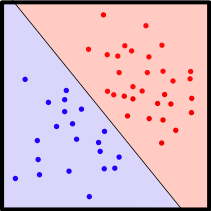
\includegraphics{linearly.png}
  \caption{Linear separability}
\end{figure}
\subsubsection{The Mathematical definition behind linear separability:}
Let $X_0$ and $X_1$ be two sets of points in an n-dimensional Euclidean space. Then $X_0$ and $X_1$
are linearly separable, if there exist $n + 1$ real numbers $w_1, w_2, \cdots, w_n, k$ such that
every point $x \in X_0$ satisfies $\sum_{i = 1}^{n}(w_i \cdot x_i) > k$ and every point $x \in X_1$
satisfies
$\sum_{i = 0}^{n}(w_i \cdot x_i) < k$ where $x_i$ is the i-th component of $x$.
\subsection{From the learning algorithm to code:}
You must create a training function with these characteristics using the previous data.
\begin{enumerate}
\item The training function guesses the outcome based on the activate function.
\item Every time the guess is wrong, the perceptron should adjust the weights.
\item After many guesses and adjustments, the weights will be correct.
\end{enumerate}
Define the activation function which at the end it is a simple binary function.
\begin{verbatim}
int activation(x)
    return (x > 0) ? 1 : -1
\end{verbatim}
Define the learning rate and a number of epochs, which is the amount of times that we are going
train the perceptron and the learning rate represents how fast our perceptron is going to learn.
\begin{verbatim}
learning_rate = 0.1
num_epochs = 100
\end{verbatim}
Train the perceptron by iterating with all the training data which in this case it is an bidimensinal
array and a simple threshold or bias.
\begin{verbatim}
for (i = 0, i < num_epochs, i++)
    for (j = 0, j < inputs.length, j++)
        sum = 0.0
        for (k = 0, k < weights.length, k++)
            sum += inputs[j][k] * weights[i]
        sum += b
        out = activation(sum)
\end{verbatim}
And at the end we only need to adjust the weights and bias from the error, so the error is so simple
it is  a subtraction, then use the error and the learning rate to update the weights and bias.
\begin{verbatim}
error = label[j] - output
for (k = 0, k < weights.length, k++)
    weights[k] += learning_rate * error * inputs[j][k]
b += learning_rate * error
\end{verbatim}
\subsection{The math behind the learning algorithm:}
Maybe now the main question is why we adjust the weights like that.
\begin{verbatim}
weights[k] += learning_rate * error * inputs[j][k]
\end{verbatim}
And the bias or threshold.
\begin{verbatim}
b += learning_rate * error
\end{verbatim}
To answer that we need to formulate a math function that represents our neuron which receives a vector
as input.
\[
  f(\vec{x}) = 
  \begin{cases}
    1 &\quad if \vec{w} \cdot \vec{x} > 0  \\
    -1 &\quad \text{otherwise} \\
  \end{cases}
\]

Where $\vec{w} = (b, w_1, \cdots, w_n)$
is the coefficients or weights, $\vec{x} = (1, x_1, \cdots, x_n)$
the input vector, so from this idea we can come up
with something like this.
\[
  y_t = 1 \implies \vec{w} \cdot \vec{x}_t > 0
\]

\[
  y_t =  - 1 \implies \vec{w} \cdot \vec{x}_t \le 0
\]
Where $(\vec{x}_t, y_t) \in \mathbb{D}$ which is the whole dataset, then from these implications
we can formulate two inequalities that
represent when the perceptron is wrong and when it is correct.
\[
  \text{Correct} \implies y_t \cdot \vec{x}_t \cdot \vec{w} > 0
\]

\[
  \text{Wrong} \implies y_t \cdot \vec{x}_t \cdot \vec{w} \le 0
\]

At the end what we want to claim is the convergence of the perceptron which looks like this.
\[
  \exists \vec{\theta}^* \in \mathbb{R}^{d} \quad|\quad y_t\vec{\theta}^*\vec{x}_t > 0,\quad
  \forall (\vec{x}_t, y_t) \in \mathbb{D}
\]
Where $\vec{\theta}^*$ is the desired vector configuration which classifies the inputs perfectly.
\section{Example:}
This is an example of how we can use the perceptron as a binary classifier, what I'm going to do
is to create a program which identifies when is a circle and when is a rectangle.
\subsection{Perceptron module in fortran:}
Firstly I made a simple perceptron module in fortran which contains the weights, a bias and with a
simple step activation function.
\begin{lstlisting}
#include <assertf.h>

module mod_perceptron
    use iso_fortran_env, only : real32, int32
 
    use assertf
    implicit none

    private
    public p_init, p_free, p_train, p_test, perceptron

    ! The type where we are going to contain the weights and bieas
    type perceptron
        real(real32) ::  b
        integer(int32) :: n     ! The amount of weights
        real(real32), pointer :: w(:) ! The weights
    end type perceptron
contains
    
    ! step: A simple activation function
    pure function step(output)
        real(real32), intent(in) :: output
        real(real32) :: step
        if (output > 0.0) then
            step = 1.0
        else
            step = 0.0
        end if
    end function step

    
    ! p_init: Receives a perceptron type and adds to it the weights
    ! and bias
    subroutine p_init(per, w, b)
        real(real32), intent(in) :: w(:), b
        type(perceptron), intent(out) :: per

        per%n = size(w)         ! Fetch the size of the array of weights
        
        ! Allocate the array of weights
        allocate(per%w(per%n))
        per%w(:) = w(:)
        per%b = b
    end subroutine p_init

    ! p_free: To free the perceptrons weights and set the size and bias
    ! to zero
    subroutine p_free(per)
        type(perceptron), intent(in out) :: per
        
        deallocate(per%w)
        per%n = 0
        per%b = 0
    end subroutine p_free
end module mod_perceptron
\end{lstlisting}
\subsection{Test and trainning function:}
Then the \textbf{test} and \textbf{training} functions.
\begin{lstlisting}
    ! p_train: To train the perceptron with some data
    subroutine p_train(per, inputs, outputs, lrate, nepochs)
        ! inout Because we are going to modify
        type(perceptron), intent(in out) :: per 
        ! The inputs and outputs to be trained
        real(real32), intent(in) :: inputs(:,:) ! Bindimensional array
        real(real32), intent(in) :: outputs(:), lrate ! Learning rate
        integer(int32), intent(in) :: nepochs        ! Num of epochs

        ! The size and the iterators
        integer(int32) :: n, i, j, k
        real(real32) :: output, error, delta
        ! Catch the amount of inputs, sizeof(inputs[1])
        n = size(inputs, 1)     
        
        do i = 1, nepochs            ! Start iterating
            do j = 1, n ! Concurrent iteration
                ! Computing the perceptron calculation
                output = per%b
                do concurrent(k = 1 : per%n)
                    output = output + per%w(k) * inputs(j, k)
                end do
                
                ! The step function
                output = step(output)

                ! Compute the error 
                error = outputs(j) - output
                delta = lrate * error

                ! Update the perceptron
                per%b = per%b + delta
                do concurrent(k = 1 : per%n)
                    per%w(k) = per%w(k) + delta * inputs(j, k)
                end do
            end do
        end do
    end subroutine p_train

    ! p_test: To test the perceptron with some inputs
    subroutine p_test(per, inputs, results)
        type(perceptron), intent(in) :: per
        real(real32), intent(in) :: inputs(:, :)
        real(real32), intent(out) :: results(:)

        ! The size and outputs
        integer(int32) :: n, i, j
        
        ! Test the perceptron
        n = size(inputs, 1)
        do concurrent(i = 1 : n)
            results(i) = per%b
            do concurrent(j = 1 : per%n)
                results(i) = results(i) + per%w(j) * inputs(i, j)
            end do
            results(i) = step(results(i))
        end do
    end subroutine p_test
\end{lstlisting}
\subsection{Main program:}



\section{Conclusion:}
Perceptrons are limited to linearly separable problems, which means that they can only learn to
classify data that can be separated by a hyperplane. However, they have been used as building blocks
for more
complex neural network architectures that can handle more complex problems.\\
Overall, perceptrons are a simple and powerful tool for building basic binary classifiers, and
they have contributed significantly to the development of artificial intelligence and machine learning.


\section{References:}
\begin{itemize}
\item Zieba, J., PhD. (2022, December 16). How Do Neurons Work? The Scientist Magazine®.
  \url{https://www.the-scientist.com/university/brush-up-how-do-neurons-work-70839}
\item Action potentials and synapses. (2017, November 9). Queensland Brain Institute - University
  of Queensland.
  \url{https://qbi.uq.edu.au/brain-basics/brain/brain-physiology/action-potentials-and-synapses}
\item Perceptrons. (n.d.). \url{https://www.w3schools.com/ai/ai_perceptrons.asp}
\item Perceptron in Machine Learning - Javatpoint. (n.d.). www.javatpoint.com.
  \url{https://www.javatpoint.com/perceptron-in-machine-learning}
\item Training a Perceptron. (n.d.). \url{https://www.w3schools.com/ai/ai_training.asp}
\item Desmedt, S. (2019, May 12). The Math behind Neural Networks: Part 1 - The Rosenblatt Perceptron.
  CodeProject.
  \url{https://www.codeproject.com/Articles/4047091
    /The-Math-behind-Neural-Networks-Part-1-The-Rosenbl}
\end{itemize}


\end{document}